\documentclass[conference]{IEEEtran}
\usepackage[justification=centering]{caption}
\usepackage{blindtext, graphicx}
\usepackage{float}

\begin{document}
\title{TeamFinder: An Application for Building Skill Based Teams}


\author{\IEEEauthorblockN{Michael Goff\IEEEauthorrefmark{1},
Shashank Jha\IEEEauthorrefmark{2},
Jingjuan Deng\IEEEauthorrefmark{3} and
Bhaskar Sinha\IEEEauthorrefmark{4}}
\IEEEauthorblockA{Department of Computer Science, North Carolina State University, \\
Raleigh, North Carolina 27606\\ 
Email: \IEEEauthorrefmark{1}magoff2@ncsu.edu \\
\IEEEauthorrefmark{2}sjha5@ncsu.edu \\
\IEEEauthorrefmark{3}jdeng8@ncsu.edu \\
\IEEEauthorrefmark{4}bsinha@ncsu.edu}}


% make the title area
\maketitle

\section{Collections}


\section{Anonymization}
In order to protect the identity of our peers we anonomized the data we pulled from the various GitHub repositories. The anonomization was performed both on the group name and the users themselves so no connection could be made back to the individuals. When gathering data each new group that was added to our databases was assigned an id number. Additionally each new user that appeared in an interaction was also assigned an id number. With personal data pulled away we can be assured that it is safe to objectively analyze the repository data without fear of offending any particular group. 

\section{Data Summary}
We have pulled data across all of the groups in the software engineering course but we decided to focus on the 3 groups with the most active repository. Below is a table of summary information about each team. 


\begin{tabular}{c|c|c|c|c}
    Team & Commits &  Issues & Milestones & Comments \\
    1 & 202 & 49 & 8 & 140 \\
    2 & 138 & 27 & 5 & 13 \\
    3 & 60 & 32 & 4 & 72 \\
\end{tabular}

It is important to note that the professor asked students to try to use GitHub as their main source of communication throughout the semester in order to generate data for this project. However, upon inspection of the data it seems that some groups talked much more than others. Team 1 maintained a high number across the board for the project by maintaining a high frequency of commits at 202 where the other groups did not keep such a high number. Perhaps team 1 prioritized frequent smaller changes while other teams preferred to make large changes at once. Another important area to judge the active level of the repository are comments. A repository with a lot of comments would imply that there was enough communication to successfully get a job done. Once again team 1 had the most with 140 comments. Team 2 had a surprising 13 comments, which almost surely implies that the team was communiciating mainly outside of GitHub. The number of issues were fairly similar among teams, with 1 having the most and 2 having the least. It could be a case of breaking issues down into smaller pieces rather than big features to implement. 

\section{Data Samples}

\section{Features}
This section will describe the various metrics we want to observe about a team to form a hypothesis about their performance. If all of these different symptoms look like they are in good shape then the project is probably going along smoothly. 

\subsection{Comments per Issue}
One feature we were interested in looking into was the number of comments per issue. The reason we wanted to look at this issue was to judge the level of collaboration between team members. If there were few comments then problems may not have been resolved in a proper manner. When paired with the time issues remain open we can gather even more insight. For instance, if an issue is open with one or less comments over an extended period of time then we can see that there is a problem with development. Another possible situation could be that the item is not a high priority, though a good team would probably leave a comment or label to make it as such. 

\subsection{Issue Duration}
Another important feature on a repository is the duration an issue remains open. Issues that have not been resolved for a long period of time may indicate features that have not been properly developed or bugs that have persisted for too long in the system. If these types of situations are not cleared up in a timely manner it can have a cumulative effect on an application. We hope to find that issues are resolved within a week of being found. This would indicate an active developer community that can quickly resolve errors in a system. If issues are left open for a longer period of time then the developers are not keeping up with the problems in the application which, over time, may lead to larger problems within the system. 

\subsection{Issue open time outside of milestone deadline}
On GitHub, issues are usually assigned to milestones. This allows developers to group similar functionality together for a release. One aspect that observes how issues and milestones are connected is whether the issue was closed before the deadline of the milestone. We predict that a good group will have most of their issues close before the due date for the milestone. 





\section{Results}
\subsection{Comments per Issue}
When pulling the number of comments per issue on the same teams we found that the average number of comments were surprisingly low across the teams as shown in figure \ref{comments_issue}. When looking at the box and whisker plot of the teams there was a telling spread of different stories across the teams. For example the majority of team 1's issues had less than 7 comments. One explanation to the lack of comments was that issues were resolved quickly and closed. Team 1 also had a lot of outlier issues that had a lot more comments than the rest of the issues. The deviance of the norm on these issues could be attributed to discussion threads that take place on the issues. It is common among groups to have a place to discuss next steps or debate over a new feature or design idea.

\begin{figure}[H]
    \centering
    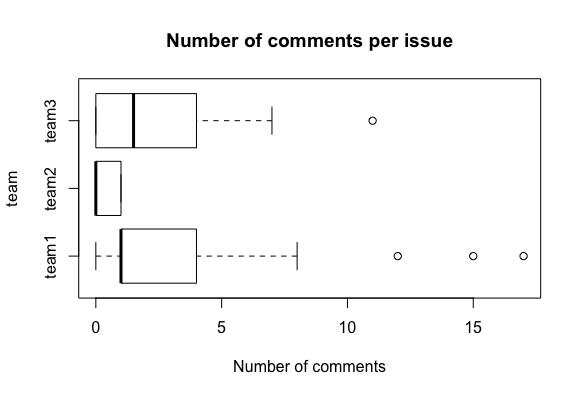
\includegraphics[width=9cm]{../AprilProject/pic/comments_per_issue.png}
    \caption{Comments per Issue across Teams}
    \label{comments_issue}
\end{figure}

Judging across all of the groups team 1 and 3 look the healthiest and team 2 looks like it is in trouble. The number of comments average is very close to zero and they did not have a single issue that contained more than 1 comment. The lack of discussion on issues indicates that there was a poor level of communication across the team. There could be some explanations to the lack of comments on issues, like another external communication channel outside of GitHub. It is possible that team 2 mainly communicated on the side and did not feel the need to document everything in issues. While this feature alone is not enough to indicate a bad team, when combined with other bad signs it could paint a more complete picture. 

\subsection{Issue Duration}
Across the teams the results were somewhat surprising when it came to issue duration, seen in figure \ref{issue_duration}. We predicted that issues would on average be open for about a week, which turned out to be mostly true except for team 3. Team 2 had an average open time of only a couple of days while team 1 had issues open for an average of 6 days. There are a lot of outlier issues on this figure though. When it comes to outlier issues, team 1 is the biggest offender. They had 7 issues that were open 30 days or longer. Surprisingly, the number of outliers did not seem to pull the average close time past a week so they must have had plenty of issues that were quickly resolved as well. 

\begin{figure}[H]
    \centering
    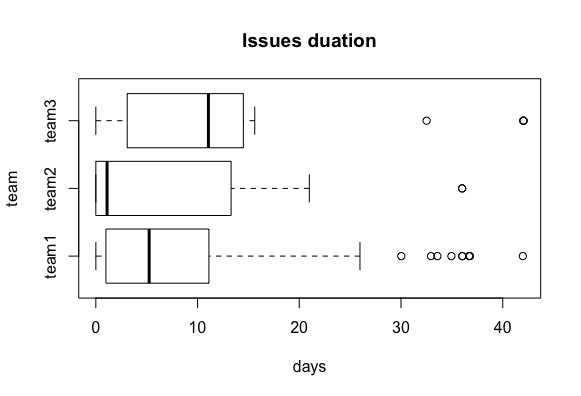
\includegraphics[width=9cm]{../AprilProject/pic/issues_duration.png}
    \caption{Duration of Issues}
    \label{issue_duration}
\end{figure}

With teams 1 and 2 quickly resolving issues it seems to indicate that they have healthier projects when it comes to turnaround on issues. Team 3 had the biggest problem with average duration. They had issues open an average of a week and a half. 

\subsection{Issues closed outside of milestone due date}
When observing the issue close date in reference to its milestone we were not very surprised by the results. The median issue was closed on the milestone due date with many of them being closed before the due date. The habits of team 2 and 3 tended to close most or almost all of their issues on the deadline of the associated milestone. Most likely as a way to clean things up after finishing that particular milestone. Team 1 had a much more varied level of issue close dates. Team 1 had most of it's issues closed before a milestone due date, however there were a good number of which that were closed after the milestone was due. 

\begin{figure}[H]
    \centering
    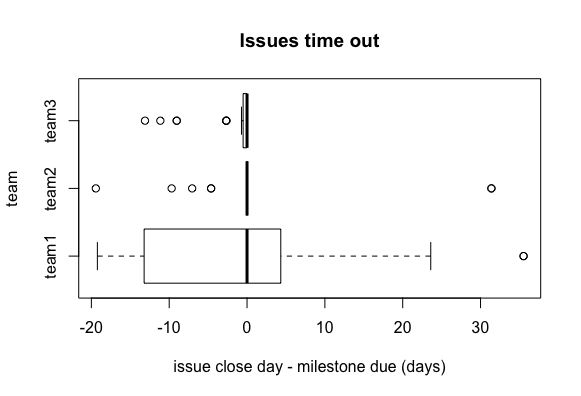
\includegraphics[width=9cm]{../AprilProject/pic/issues_timeout.png}
    \caption{Issue Timeout}
    \label{issue_timeout}
\end{figure}


Except for a few outlier issues that were closed long after the milestone due date, all of the teams were pretty healthy regarding this metric. Based off of the data in figure \ref{issue_timeout} we think that issues were not often closed in a timely manner or the groups were big on procrastinating until the deadline. 

\subsection{Milestone Timeline}
While observing the milestone timeline it was observed that out of the three teams, Team3 did not create enough issues throughout the project and did not set due dates for those milestones as well which is quite different to what was observed for the other two teams. 


\begin{figure}[H]
    \centering
    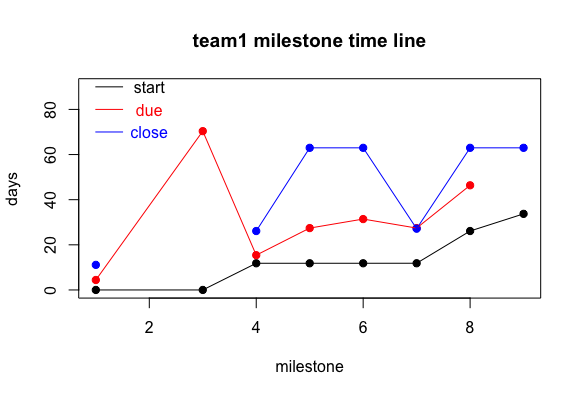
\includegraphics[width=9cm]{../AprilProject/pic/team1_milestone_time.png}
    \caption{Team 1 Milestone Time}
    \label{team1_milestone_time}
\end{figure}

Team1 created the most milestones and set a due date for almost all of them. Team2 as well created milestones throughout the project and set due dates for them.



\begin{figure}[H]
    \centering
    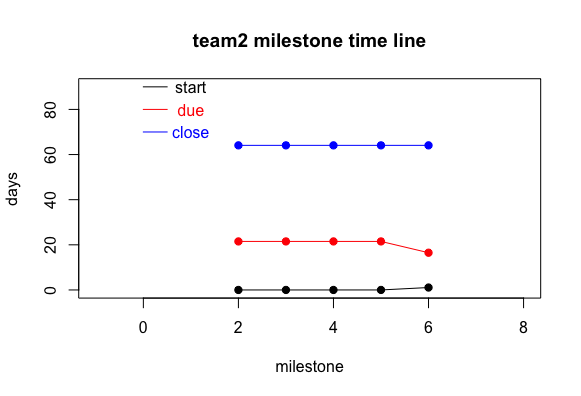
\includegraphics[width=9cm]{../AprilProject/pic/team2_milestone_time.png}
    \caption{Team 2 Milestone Time}
    \label{team2_milestone_time}
\end{figure}


Regarding the closing time of the milestones across all teams it was observed that almost all milestones were closed after the due date set for them. For team 1, only one milestone was closed. Team 1 and 2 closed almost all of their milestones.

\begin{figure}[H]
    \centering
    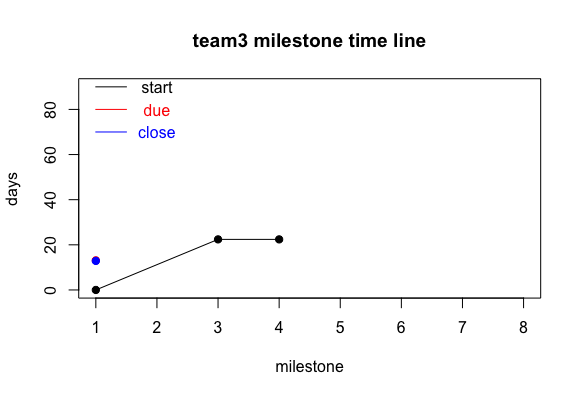
\includegraphics[width=9cm]{../AprilProject/pic/team3_milestone_time.png}
    \caption{Team 3 Milestone Time}
    \label{team3_milestone_time}
\end{figure}

\subsection{Issues assigned to member having comments}



\begin{figure}[H]
    \centering
    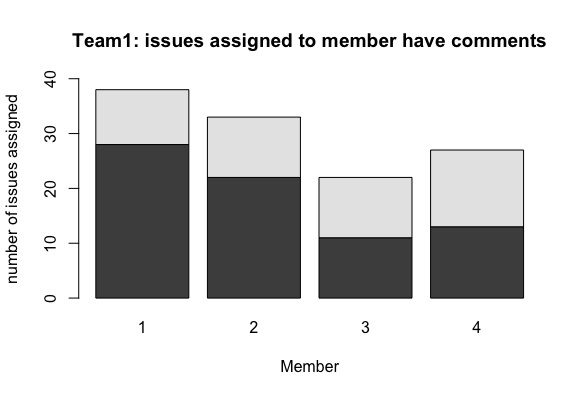
\includegraphics[width=9cm]{../AprilProject/pic/team1_user_issue_comments.png}
    \caption{Team 1 User Issue Comments}
    \label{team1_issue_comment}
\end{figure}

\begin{figure}[H]
    \centering
    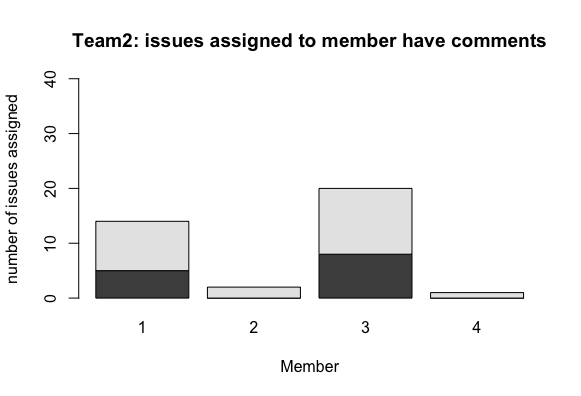
\includegraphics[width=9cm]{../AprilProject/pic/team2_user_issue_comments.png}
    \caption{Team 2 User Issue Comments}
    \label{team2_issue_comment}
\end{figure}

\begin{figure}[H]
    \centering
    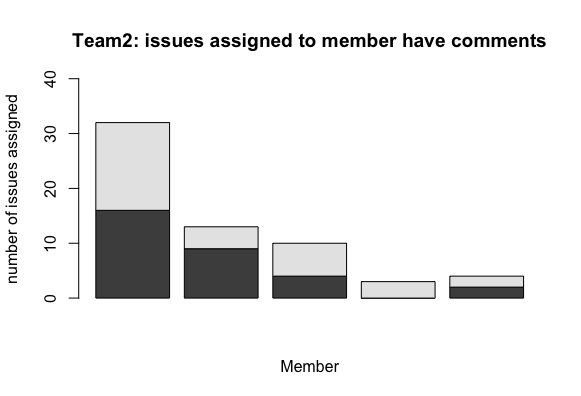
\includegraphics[width=9cm]{../AprilProject/pic/team3_user_issue_comments.png}
    \caption{Team 3 User Issue Comments}
    \label{team3_issue_comment}
\end{figure}
\section{Bad Smells Detector}
\section{Early Warning}

\end{document}